\documentclass[a4paper, 12pt]{scrartcl}
% A4 Papier, 12pt Schriftgröße
% scriptartcl, weil article für englischsprachigen Raum optimiert



% --- EINSTELLUNGEN FÜR DEUTSCHE DOKUMENTE:
\usepackage[ngerman]{babel}
% new german (neue deutsche Rechtschreibung)

\usepackage[utf8]{inputenc}
% utf8-Eingabe (Umlaute etc...)

\usepackage[T1]{fontenc}
% damit im erstellten PDF auch nach Wörtern mit Umlauten gesucht werden kann

\usepackage{csquotes}
% für deutsche Anführungsstriche

\usepackage[addtotoc]{abstract}


\usepackage{graphicx}
% für Bilder

\title{End-to-end-Learning Ansatz für autonomes Fahren im Miniatur Wunderland}
\author{Nils-Ole Bickel, Michel Brüger}
\date{\today}

\begin{document}
	
\maketitle
% Erstellt den Titel, entsprechend den Angaben in der Präambel



\begin{abstract}	
Für autonome Miniaturfahrzeuge wird ein End-to-End-Learning-Verfahren entwickelt. Vom Miniaturfahrzeug aufgenommene Kamerabilder werden per WLAN an einen \emph{Raspberry Pi} übertragen. Im Voraus wird ein Neuronales Netz mit Kamerabildern mehrerer Trainingsfahrten im \emph{Miniaturwunderland}, bei denen das normale Lenksystem der Anlage verwendet wird, und den dazugehörigen Lenkwinkeln der Vorderachse des Miniaturfahrzeugs trainiert. 

Im Testbetrieb wird dann mittels einer per USB an den \emph{Raspberry Pi} angeschlossenen Tensor Processing Unit (\emph{Google Coral}), unter Verwendung von \emph{Tensorflow Lite}, auf einem \emph{Linux}-Betriebssystem, von dem Neuronalen Netz der zur jeweiligen Situation passende Lenkwinkel berechnet.
Als Teststrecke wird wie auch beim Training das \emph{Miniaturwunderland} benutzt.
\end{abstract}
	

%\tableofcontents
% Automatisch erstelltes Inhaltsverzeichnis
% zweimal kompilieren, damit Änderungen korrekt angezeigt werden

\newpage
% neue Seite anfangen, damit Titel und Inhaltsverzeichnis auf eigener Seite stehen
	
	\section{Einleitung}
	Die für Machine Learning benötigte Hardware wird im Lauf der Zeit immer kleiner und effizienter. Bezug nehmend auf bereits geleistete Forschung zum Thema End-to-End-Learning für autonome Fahrzeuge \cite{article} beschreiben wir in diesem Artikel die Möglichkeit die Hardware für dieses Vorhaben derart zu minimieren, dass es möglich ist ein Miniaturfahrzeug \cite{article2} autonom durch das Miniaturwunderland fahren zu lassen. Dabei handelt es sich nach eigenen Angaben um die "größte Modelleisenbahn der Welt", im Maßstab 1:87 (H0), wobei sich außer Zügen auch Autos und Schiffe autonom durch die Modelllandschaft bewegen. Es werden dort große Bereiche urbanen sowie auch Ländlichen Raums detailliert nachgebildet.
	
	 Die Besonderheit des End-to-End-Learning-Ansatzes ist, dass das CNN nicht auf einzelne Features trainiert werden muss, sondern anhand der Trainingsbilder und der dazugehörigen Sensordaten direkt den Lenkwinkel zur jeweiligen Fahrsituation lernt. 

	

	\section{Hardware}
		\subsection{Raspberry Pi 4}
		Für die Berechnung des benötigten Lenkwinkels sendet das Auto die Kameradaten an einen \emph{Raspberry Pi 4}. 
		
		Die Auslagerung auf den \emph{Raspberry Pi 4} hat mehrere Vorteile. Der \emph{Raspberry Pi 4} stellt deutlich potentere Hardware zur Verfügung im Vergleich zum Auto. Er verfügt über zwei USB-3-Anschlüsse. Diese sind wichtig um das volle Potential aus dem \emph{Google Coral USB Accelerator} herauszuholen. Außerdem bietet er die Möglichkeit vollwertige Linux-Betriebssysteme zu installieren, was die Verwendung der für die AI-Lenkwinkel-Voraussagung notwendigen Software ermöglicht.
		
		Im Vergleich zu anderen Computern war die Größe des \emph{Raspberry Pi 4} ein entscheidender Faktor. Der kleine Formfaktor ermöglicht es den \emph{Raspberry Pi 4} leicht im \emph{Miniatur Wunderland} zu verstecken. Die Möglichkeit, ihn über eine Powerbank per USB-C zu laden, macht dies noch leichter, da man nicht noch ein Kabel zu einem Stromanschluss verlegen muss.
		
		
		\subsection{Google Coral USB Accelerator}
		Der \emph{Google Coral USB Accelerator} ist ein Tensor-Prozessor in Form eines USB-Sticks, der an einen Rechner wie den \emph{Raspberry Pi} angeschlossen werden kann, um die Machine Learning Operationen schnell und besonders energieeffizient durchzuführen. Dies kann der \emph{Raspberry Pi 4} zwar auch alleine bewerkstelligen, der \emph{Google Coral USB Accelerator} ist dabei aber deutlich schneller. Bei spontanen Vergleichen konnten wir eine 14-fache Geschwindigkeit bei der Objekterkennung in Bildern feststellen.

	
		\subsection{Der Trainingsrechner}
		Das Netz wurde auf einem der Laborrechner trainiert. Dieser verfügt über eine \emph{Nvidia Geforce GTX 1050 Ti} Grafikkarte, welche den Trainingsprozess deutlich beschleunigt, im Vergleich zum Training mit der CPU.	
	
	\section{Software}
		\subsection{Auf dem Raspberry Pi verwendete Software}
			\subsubsection{Raspbian}
			Als Betriebssystem auf dem \emph{Raspberry Pi 4} wird \emph{Raspbian Buster} verwendet. Dabei handelt es sich um eine auf Debian basierende Linux-Distribution.
			
			
			\subsubsection{Python}
			Standardmäßig ist \emph{Python 3.7} in \emph{Raspbian Buster} enthalten. Dies ist für die Verwendung des \emph{Google Coral USB Accelerator} mit \emph{Tensorflow Lite} ausreichend.
			
			\subsubsection{Edge TPU runtime}
			Die \emph{Edge TPU runtime} wird für die Kommunikation mit dem \emph{Google Coral USB Accelerator} benötigt.
			
			Während der Installation der \emph{Edge TPU runtime} kann man auswählen, ob man den \emph{Google Coral USB Accelerator} mit Standardgeschwindigkeit oder maximaler Geschwindigkeit (2x Standard) betreiben möchte. Da sich bei unseren Versuchen mit Standardgeschwindigkeit herausgestellt hat, dass der \emph{Raspberry Pi 4} bei der Vorbereitung der Bilder überhitzt, ist eine Installation mit maximaler Geschwindigkeit überflüssig.
			
			\subsubsection{Tensorflow Lite Library für Python}
			Da auf dem \emph{Raspberry Pi 4} lediglich \emph{Tensorflow Lite} Modelle ausgeführt werden sollen reicht die Installation des \emph{Tensorflow Lite interpreter} anstelle aller Tensorflow Pakete.
			
				
		
		\subsection{Auf dem Trainingsrechner verwendete Software}
		Auf den Labor-PCs ist \emph{Anaconda} installiert.
			\subsubsection{Anaconda}
			In \emph{Anaconda} können unter Verwendung von \emph{Conda} virtuelle Umgebungen (Environments) erstellt werden, in denen voneinander unabhängige \emph{Python}-Installationen existieren können. 
			
			In unserer virtuellen Umgebung wird \emph{Python 3.7} und die aktuelle Version von \emph{Tensorflow} mit GPU Support installiert.
			
			Beim Training wird ein normales \emph{Tensorflow} Modell trainiert. Da auf dem  \emph{Raspberry Pi 4} nur \emph{Tensorflow Lite} Modelle ausgeführt werden sollen wird dies mit Hilfe des \emph{TFLiteConverter} von  \emph{Tensorflow}  in ein \emph{Tensorflow Lite} Modell umgewandelt.
			
	
			
		\section{Das Netz}
			\subsection{Implementierung}
			Das Netzwerk besteht aus 11 Layern. Bei 6 davon handelt es sich um Convolutional Layer. Die anderen 5 sind fully-connected Layer. Die Convolutional Layer sind für die Featureerkennung verantwortlich. Die ersten 4 haben einen Kernel der Größe 5x5 und Strides der Größe 2x2. Die anderen Convolutional Layer haben einen Kernel der Größe 3x3 und Strides der Größe 1x1. Anschließend kommen die 5 fully-connnnected Layer. Das Ergebnis beschreibt den Lenkwinkel. \\ \\
			Als Vorlage für das Netzwerk wurde das Netzwerk aus dem Paper \cite{article} verwendet. Unsere Bilder haben eine Größe von 300x800. Dies ist deutlich größer als im Paper, weshalb das Netzwerk um weitere Layer, auf das oben beschriebene, erweitert wurde.
		
			\begin{verbatim}		
_________________________________________________________________
Layer (type)                 Output Shape              Param #   
=================================================================
conv2d (Conv2D)              (None, 148, 398, 32)      2432      
_________________________________________________________________
conv2d_1 (Conv2D)            (None, 72, 197, 64)       51264     
_________________________________________________________________
conv2d_2 (Conv2D)            (None, 34, 97, 64)        102464    
_________________________________________________________________
conv2d_3 (Conv2D)            (None, 15, 47, 64)        102464    
_________________________________________________________________
conv2d_4 (Conv2D)            (None, 13, 45, 64)        36928     
_________________________________________________________________
conv2d_5 (Conv2D)            (None, 11, 43, 64)        36928     
_________________________________________________________________
flatten (Flatten)            (None, 30272)             0         
_________________________________________________________________
dense (Dense)                (None, 1000)              30273000  
_________________________________________________________________
dense_1 (Dense)              (None, 100)               100100    
_________________________________________________________________
dense_2 (Dense)              (None, 50)                5050      
_________________________________________________________________
dense_3 (Dense)              (None, 10)                510       
_________________________________________________________________
dense_4 (Dense)              (None, 1)                 11        
=================================================================
Total params: 30,711,151
Trainable params: 30,711,151
Non-trainable params: 0
_________________________________________________________________
			\end{verbatim}
			
			\subsection{Berechnung der Lenkwinkel}
			Das Auto besitzt einen Hall Sensor an der Vorderachse. Statt eines Lenkwinkels in Grad wird deshalb der Lenkwinkel mit den Werten des Hall Sensors approximiert. Genauer stellt die Länge des Vektors(X, Y) vom Hall Sensor den Lenkwinkel in unserer Anwendung dar.
			
			\subsection{Training}
				\subsubsection{Trainingsdaten}
				Die Trainingsdaten wurden mit Hilfe des Autos aufgenommen. Das Auto ist entlang eines Drahtes nach dem Faller Car-System durch das Miniatur Wunderland gefahren. Dabei wurden Video-Stream und zugehörige Werte des Hall Sensors aufgezeichnet. Die obere Hälfte des Bildausschnitts wird verworfen. Dies führt dazu, dass großteils die Straße auf den Bildern zu sehen ist [Abbildung \ref{fig:trainigsdaten}]. Die Hoffnung ist, dass dadurch das Netzwerk nicht durch Häuser oder Deckenelemente im Miniatur Wunderland abgelenkt wird und somit allgemeiner eingesetzt werden kann. \\ \\
				Die Bilder werden als BGR-Bilder mit 3 Kanälen zusammen mit den Daten zum Lenkwinkel in einer H5-Datei gespeichert. Dabei ist zu beachten, dass die Bilddaten bereits als float32 Werte gespeichert werden. Sonst muss dieser rechenaufwändige Schritt während des Trainings durchgeführt werden. Eine Normierung der Bilddaten auf einen Wert zwischen 0 und 1 könnte zu einer Verbesserung der Ergebnisse vom Netzwerk führen. Allerdings würde es die Zeit, bis ein Bild bearbeitet wurde, deutlich erhöhen. Aufgrund dessen haben wir uns gegen eine Normierung entschieden.
				
				\begin{figure}[h!]
				   	 \centering
   					 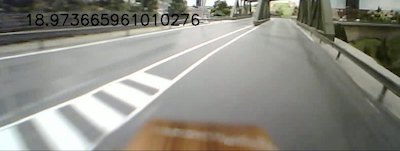
\includegraphics{Trainingsdaten-1}
					 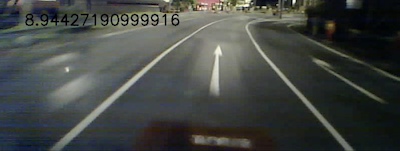
\includegraphics{Trainingsdaten-2}
					 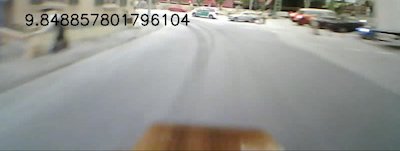
\includegraphics{Trainingsdaten-3}
  					  \caption{Beispiele aus den Trainingsdaten mit eingeblendeten Metadaten.}
 					   \label{fig:trainigsdaten}
				\end{figure}
				
				\subsubsection{Optimierung}
				Das Netzwerk wird dahingehend Trainiert die durchschnittlichen Quadratischen Abweichung (mse) zwischen dem Ergebnis des Netzes und den gemessenen Daten zum Lenkwinkel zu minimieren. Dies führt dazu, dass große Abweichungen besonders stark Gewichtet werden und kleinere nur geringer. 
		
	\section{Bewertung}
	Im Rahmen der Ausarbeitung konnte das System noch nicht vollständig getestet werden. Dementsprechend können keine Aussagen über Genauigkeit und Eignung des Netzes getätigt werden. \\ \\
	Das Netz wurde bereits in einer ähnlichen Anwendung getestet. Hierbei wurden Kamerabilder eines Handys an den \emph{Raspberry Pi 4} mit \emph{Google Coral USB Accelerator} gesendet und von einem \emph{Tensorflow Lite} Model ausgewertet. Das Model war darauf trainiert, statt einem Lenkwinkel, die aktuelle Ausrichtung des Handys zu bestimmen. Das Handy war hierbei statisch und konnte sich nur um die eigene Achse drehen. Die aussagen des Netzwerks waren bereits vielversprechend. Es ist allerdings aufgefallen, dass der \emph{Raspberry Pi 4} bereits nach kurzer Zeit überhitzt. Für zukünftige Tests sollte dementsprechend eine Kühlung des \emph{Raspberry Pi 4} beachtet werden.
	
		\subsection {Ausblick}
		Weiterführend muss die Implementierung des Systems vervollständigt werden und auf Genauigkeit geprüft werden. Anpassungen an dem Aufbau des Netzes könnten hierbei notwendig sein. Des weiteren muss man Möglichkeiten hinzufügen eine Route zu planen, sodass das Auto an Kreuzungen variable agieren kann.
		
	
		
	\bibliography{references}
	\bibliographystyle{alpha}
	\nocite{*}
	
\end{document}